\documentclass[11pt,a4paper]{article}

\usepackage[T1]{fontenc}
\usepackage[utf8]{inputenc}
\usepackage[a4paper,margin=1.8cm]{geometry}
\usepackage{amsmath,amssymb}
\usepackage{booktabs,longtable,array,tabularx}
\usepackage{graphicx}
\usepackage{microtype}
\usepackage{xcolor}
\usepackage{hyperref}

\hypersetup{colorlinks=true,linkcolor=blue,citecolor=blue,urlcolor=blue}

\graphicspath{{./images/}}

\renewcommand{\thesection}{S\arabic{section}}
\renewcommand{\thesubsection}{S\arabic{section}.\arabic{subsection}}
\renewcommand{\thetable}{S\arabic{table}}
\renewcommand{\thefigure}{S\arabic{figure}}
\newcommand{\code}[1]{\texttt{#1}}
\newcommand{\modelname}{\texttt{minimocas}}
\setlength{\tabcolsep}{4pt}
\renewcommand{\arraystretch}{1.12}

\title{Supplementary Material for\\
\emph{Large-scale traffic flow reconstruction from heterogeneous mobility sensors}}
\author{Federico Bellisardi, Chiara Mizzi, Alessandro Fabbri and Armando Bazzani}
\date{}

\begin{document}
\maketitle

\noindent This supplementary material documents the meaning of the data
layers, model variables, data-assimilation logic, validation metrics and webserver architecture supporting the main manuscript. It deliberately avoids listing repository paths; the focus is on what each component represents, why it is needed, and how it enters the reconstruction workflow. Numerical choices are reported together with their interpretation. Some of them are inherited from the temporal resolution of the observations, some are computational choices that stabilize the simulator, and some are reporting thresholds used to choose clear representative examples for the paper figures.

\section{Data Layers}
\label{sec:data-layers}

The reconstruction combines four observational layers and one derived road support. Their roles are distinct and are not interchangeable (Table~\ref{tab:data-layers}). The mobile-phone layer is the only one that describes regional demand at population scale, but it is too coarse to say which road was used. The road graph provides the missing physical support for route assignment. Coils provide accurate local counts, but only where a sensor exists. Viasat is spatially richer than coils, but it is a probe sample rather than a total-count system. The reconstructed link-flow table is therefore not a direct observation; it is the result of combining these partial views under the explicit model assumptions described below.

\begin{longtable}{@{}p{0.23\linewidth}p{0.21\linewidth}p{0.45\linewidth}@{}}
\caption{Meaning and role of the data layers.}
\label{tab:data-layers}\\
\toprule
Layer & Spatial/temporal support & Meaning in the workflow \\
\midrule
\endfirsthead
\toprule
Layer & Spatial/temporal support & Meaning in the workflow \\
\midrule
\endhead
\bottomrule
\endfoot
Mobile-phone OD activity &
Municipality pairs, hourly profiles &
Population-scale demand. It defines where trips are generated and how demand
changes over the day, but it does not identify the road sequence used by each
trip. \\
Road graph &
Directed polylines and nodes &
Physical support on which demand is assigned. It stores connectivity,
directionality, segment length and turn constraints. \\
MTS inductive loop detectors (coils) &
Fixed points, 15-min counts &
Local direct traffic measurements. They anchor the simulation and drive the
data assimilation where observed counts are available. \\
Viasat GPS telemetry &
Matched road links, hourly counts &
Independent validation layer. Because it samples only part of the vehicle
population, it is compared with simulation after estimating link-specific
penetration. \\
Derived link-flow tables &
Directed road links, hourly counts &
Simulation output after optional data assimilation. These tables are the operational
link-level reconstruction used for maps, validation and webserver delivery. \\
\end{longtable}

\subsection{Demand Structure}

The weekday and weekend OD matrices are highly concentrated. This motivates using the observed spatial demand instead of injecting uniform trips across the region. The total-flow values in Table~\ref{tab:od-structure} are the activity weights entering the demand generator after aggregation over the selected January 2020 period. They should be interpreted as relative mobility mass rather than as direct vehicle counts. Positive cells count municipality pairs with non-zero activity. The Gini coefficient and top-share columns quantify concentration: values close to 0.8 and a top-1\% share above 0.4 mean that a small number of OD relations dominate the signal. This is why the model uses observed high-demand centres explicitly and treats weakly observed endpoints through random classes instead of forcing unreliable low-count OD pairs into deterministic routes.

\begin{table}[htbp]
\centering
\caption{Structure of the weekday and weekend (Saturday--Sunday) OD matrices.}
\label{tab:od-structure}
\begin{tabular}{@{}lrrrrr@{}}
\toprule
Period & Total flow & Positive cells & Gini & Top 10\% share & Top 1\% share \\
\midrule
Weekdays & 2,665,186 & 87,212 & 0.788 & 0.708 & 0.448 \\
Weekends & 2,198,516 & 87,447 & 0.777 & 0.690 & 0.432 \\
\bottomrule
\end{tabular}
\end{table}

The ranking in Table~\ref{tab:city-ranking} is used only to describe the heterogeneity of municipal activity and to identify the dominant urban centres. The last-ranked municipalities have mean activity equal to one because they are at the residual tail of the aggregated demand table. They are kept in the descriptive statistics, but the simulator does not assume that such low-activity entries carry enough information to define precise origin--destination routes on their own.

\begin{table}[htbp]
\centering
\caption{Municipality activity ranking used to define high-demand centres.}
\label{tab:city-ranking}
\begin{tabular}{@{}rlr@{\qquad}rlr@{}}
\toprule
\multicolumn{3}{c}{Highest activity} & \multicolumn{3}{c}{Lowest activity} \\
\cmidrule(r){1-3}\cmidrule(l){4-6}
Rank & Municipality & Mean points & Rank & Municipality & Mean points \\
\midrule
1 & Bologna & 345,267 & 519 & Montecalvo in Foglia & 1 \\
2 & Modena & 176,166 & 520 & Porto San Giorgio & 1 \\
3 & Parma & 158,440 & 521 & Trento & 1 \\
4 & Ravenna & 147,772 & 522 & Montepulciano & 1 \\
5 & Rimini & 144,696 & 523 & Vescovato & 1 \\
6 & Reggio nell'Emilia & 139,849 & 524 & Tortona & 1 \\
7 & Ferrara & 103,067 & 525 & Aviano & 1 \\
8 & Piacenza & 92,678 & 526 & Malborghetto Valbruna & 1 \\
9 & Forl\`i & 86,078 & 527 & Bolzano & 1 \\
10 & Cesena & 78,582 & 528 & Grottammare & 1 \\
\bottomrule
\end{tabular}
\end{table}

\subsection{Sensor and Telemetry Coverage}

Table~\ref{tab:data-volumes} reports data volume in terms of records, variables and physical interpretation. The 528 municipalities define the areal units of the demand layer. The 292 traffic stations are sparse compared with the road graph, so data assimilation has to be local and directional rather than a global rescaling of the whole network. The 5,760 rows of the 2020 coil table correspond to 60 days at 15-min resolution; each day contributes 96 samples per direction. The Viasat campaigns contain hundreds of thousands of hourly link observations, but the 4,186 matched road identifiers are still only a subset of the regional graph. This justifies using Viasat for temporal-profile validation and not as a complete observation layer.

\begin{table}[htbp]
\centering
\caption{Observed data volumes used by the paper workflow.}
\label{tab:data-volumes}
\begin{tabular}{@{}lrrp{0.35\linewidth}@{}}
\toprule
Layer & Records & Variables & Interpretation \\
\midrule
Municipality activity table & 528 & 5 & Ranked source and destination
activity over municipalities. \\
Coil registry & 292 & 5 & Geographical catalogue of traffic-count stations. \\
Coil-to-road matching & 292 & 9 & Association between each traffic station
and a graph polyline. \\
February--March 2020 coil table & 5,760 & 496 & Fifteen-minute directional
traffic counts used for the coil-282 comparison and data-assimilation support. \\
Viasat 2020 campaign & 803,904 & 10 & Hourly GPS link-flow observations over
4,186 matched road identifiers. \\
Viasat 2021 campaign & 703,416 & 10 & Hourly GPS link-flow observations over
the same matched road universe. \\
\bottomrule
\end{tabular}
\end{table}

\section{Simulation Runs and Source Classes}
\label{sec:simulation-runs}

The final validation archive contains sixteen daily simulations, eight in February 2020 and eight in June--July 2021. The two periods were selected because independent Viasat validation campaigns are available for those dates. Viasat is not used to configure or assimilate the simulations; it provides the held-out probe layer against which simulated link profiles are compared. The periods are not intended to span all seasonal variability; they provide two well-defined weeks in which reconstructed link flows and GPS probe flows can be compared consistently.

Every run uses a 10 s integration time step and writes hourly outputs. The 10 s step is short enough to move agents through short links without creating coarse jumps at intersections, while remaining computationally light for regional daily runs. Hourly output is used because both the mobile-phone demand profiles and the validation figures are expressed at hourly scale; it also reduces noise relative to 15-min sensor counts while preserving morning, midday and evening traffic structure. The source count changes by day because the OD generator activates only demand components present in the selected daily schedule.

\begin{longtable}{@{}llp{0.36\linewidth}@{}}
\caption{Archived daily simulation configurations, summarized by meaning
rather than file name.}
\label{tab:daily-runs}\\
\toprule
Date & Sources & Output support \\
\midrule
\endfirsthead
\toprule
Date & Sources & Output support \\
\midrule
\endhead
\bottomrule
\endfoot
2020-02-10 & 758 & Hourly directed links \\
2020-02-11 & 740 & Hourly directed links \\
2020-02-12 & 762 & Hourly directed links \\
2020-02-13 & 736 & Hourly directed links \\
2020-02-14 & 722 & Hourly directed links \\
2020-02-15 & 758 & Hourly directed links \\
2020-02-16 & 980 & Hourly directed links \\
2020-02-17 & 758 & Hourly directed links \\
2021-06-28 & 763 & Hourly directed links \\
2021-06-29 & 744 & Hourly directed links \\
2021-06-30 & 766 & Hourly directed links \\
2021-07-01 & 740 & Hourly directed links \\
2021-07-02 & 726 & Hourly directed links \\
2021-07-03 & 763 & Hourly directed links \\
2021-07-04 & 983 & Hourly directed links \\
2021-07-05 & 763 & Hourly directed links \\
\end{longtable}

The slightly larger source counts on Sundays arise from the way residual weekend mobility is represented: when the observed OD structure is less dominated by commuting pairs, more source components are needed to preserve regional coverage. This does not mean that Sunday traffic is necessarily larger than weekday traffic; it means that the demand generator uses a larger set of active source definitions to represent a more diffuse mobility pattern.

\begin{table}[htbp]
\centering
\caption{Source-class counts across the archived simulations.}
\label{tab:source-classes}
\begin{tabular}{@{}lrrrp{0.33\linewidth}@{}}
\toprule
Class & Min/day & Max/day & Total & Endpoint logic \\
\midrule
Fixed municipality OD & 563 & 804 & 9,843 & Observed source and observed
destination. \\
Fixed province OD & 55 & 78 & 1,003 & Province-level source and destination. \\
Source-random & 50 & 50 & 800 & Observed source, sampled destination. \\
Random-destination & 50 & 50 & 800 & Sampled source, observed destination. \\
Random-random & 1 & 1 & 16 & Both endpoints sampled from the modelled region. \\
\bottomrule
\end{tabular}
\end{table}

The fixed municipality OD class dominates because it is the part of the demand where both endpoints are directly observed. The two one-sided random classes are kept at 50 sources per day so that residual mobility can enter and leave the main observed centres without overwhelming the empirical OD matrix. The single random--random source is a low-intensity background component: it prevents the model from suppressing trips with neither endpoint in the dominant observed set, but it is deliberately small so that it cannot create an artificial uniform traffic field.

\section{\modelname{} Model Details}
\label{sec:model-details}

\modelname{} is an agent-based road simulator. Vehicles are represented by
agents that move on directed polylines, choose a next node at junctions and accumulate link-level counts. The model state is summarized in Table~\ref{tab:pawn-vars}. The implementation is intentionally mesoscopic in spirit: agents are individual vehicles, but the objective is not to reproduce lane-changing details or second-by-second car-following trajectories. Instead, the model produces a directional link-by-time flow field that can be locally constrained by fixed counters and validated against held-out probe data.

\begin{longtable}{@{}p{0.25\linewidth}p{0.18\linewidth}p{0.47\linewidth}@{}}
\caption{Main vehicle-agent state variables.}
\label{tab:pawn-vars}\\
\toprule
State variable & Type/unit & Role \\
\midrule
\endfirsthead
\toprule
State variable & Type/unit & Role \\
\midrule
\endhead
\bottomrule
\endfoot
Identifier & integer & Distinguishes each simulated vehicle. \\
Status & categorical & Tracks whether the vehicle is active, completed,
waiting, queued or interacting with transport logic. \\
Current road link & polyline id & Link occupied by the vehicle at the
current time step. \\
Position on link & m & Longitudinal coordinate along the occupied link. \\
Signed speed & m s$^{-1}$ & Magnitude gives speed; sign encodes direction. \\
Destination & node id & Current graph node pursued by the routing rule. \\
Previous and next node & node ids & Junction state used to move between
links. \\
Route-deviation parameter & probability & Controls whether the vehicle
follows or departs from the precomputed best path. \\
Distance and time counters & m, s & Accumulate travelled distance, trip time
and lifetime. \\
\end{longtable}

Best paths are computed on a weighted graph with a Dijkstra-style engine. In the archived validation runs the routing weight reduces to polyline length, while forbidden turns are still excluded. The movement update also contains a density-dependent speed rule:
\begin{equation}
v_p^{\rm target} =
\begin{cases}
v_{\rm crit}, & \rho_p > \rho_{\rm crit},\\
(1-\rho_p/\rho_{\rm crit})v_p, & \rho_p \leq \rho_{\rm crit},
\end{cases}
\qquad
v_p^{\rm target}\geq v_{\rm crit}.
\end{equation}
The validation configuration uses $\rho_{\rm crit}=3/4.20$~m$^{-1}$ and
$v_{\rm crit}=10/3.6$~m~s$^{-1}$.

The critical density corresponds to a compact but still interpretable spacing: roughly three vehicles over 4.2~m in the internal density convention used by the simulator. Its role is not to calibrate a detailed fundamental diagram; it prevents unrealistically high speeds when many agents occupy the same link. The critical speed is 10~km~h$^{-1}$, converted to SI units, and acts as a lower operational speed in congested conditions. The rule should therefore be read as a stabilizing traffic-flow constraint rather than as a fitted car-following law.

\begin{table}[htbp]
\centering
\caption{Numerical parameters and switches in the archived validation runs.}
\label{tab:parameters}
\begin{tabularx}{\linewidth}{@{}l l X@{}}
\toprule
Parameter & Value & Role \\
\midrule
Integration step & 10 s & Numerical simulation step. \\
Output sampling & 3600 s & Temporal resolution of saved link counts. \\
Source activation & 30 s & Interval at which new vehicles are generated. \\
State grid cell & 5000 m & Spatial scale of gridded state output. \\
Cartographic index cell & 10000 m & Spatial index used for graph lookup. \\
Length routing weight & 1.0 & Makes routing cost proportional to length. \\
Speed routing weight & 0.0 & Disables speed-dependent routing in archived runs. \\
Initial speed range & 15--25 m s$^{-1}$ & Sampling range for generated vehicles. \\
Random-endpoint time budget & 5600 s & Maximum time field used by random
source classes. \\
Unique-link output & active & Saves the directional link counts used in the
paper. \\
\bottomrule
\end{tabularx}
\end{table}

The values in Table~\ref{tab:parameters} reflect a compromise between temporal fidelity and reproducibility. A 10 s integration step is small relative to the one-hour saved output and keeps route progression smooth. The 3600 s sampling interval is chosen because the OD demand and Viasat validation are analysed hourly; using a finer output would mostly preserve sensor noise rather than add information to the paper figures. The 30 s source-activation interval spreads injected agents over each hour instead of creating a single burst at the hour boundary. The 5000 m state grid and 10000 m cartographic index are lookup scales used to organize regional graph operations; they are much larger than individual road links, so they do not define the resolution of the final traffic field. Setting the length routing weight to 1.0 and the speed routing weight to 0.0 makes route choice depend on path length in the archived runs. This choice avoids mixing route assignment with uncertain speed calibration when the main objective is to validate link-flow profiles. The 15--25 m s$^{-1}$ initial-speed range covers typical extra-urban speeds before density updates. The 5600 s random-endpoint time budget is a soft bound used when sampling residual trip endpoints: it allows trips longer than a one-hour commute but avoids generating unrealistic cross-region random journeys as the dominant residual class.

\section{Coil-based Data Assimilation}
\label{sec:post-correction}

The data-assimilation step adjusts simulated unique-link counts using MTS coil residuals. Directional coil columns are mapped to cartographic
\code{IN}/\code{OUT} directions. The archived validation runs were assimilated with the version of the code dated 30 March 2023; rerunning that version on the stored inputs reproduces the archived 10 February 2020 table to machine precision. In that version, gaps in an observed coil table are filled by linear interpolation in time, and when no observed table covers the simulated day (the 2021 runs) the weekday-specific seasonal average of each coil is used. The operational code now in the webserver fills missing values with seasonal weekday averages that combine the most recent year and earlier years with inverse standard-deviation weights.

For a coil-associated directed link $i$, let $u_i(h)$ be the unique-link count, $b_i(h)$ the simulated virtual-barrier count and $c_i(h)$ the measured coil count. The data-assimilation step estimates a barrier-to-unique relation and a local relative residual,
\begin{equation}
r_i(h)=\frac{b_i(h)}{\max(u_i(h),1)}, \qquad
\Delta_i(h)=
\frac{c_i(h)r_i(h)-b_i(h)}{\max(b_i(h),1)}.
\end{equation}
This residual becomes the additive increment $\delta_i(h)=u_i(h)\Delta_i(h)$ on the local directed link, so that the assimilated count equals $c_i(h)$ whenever $u_i,b_i\ge1$, and is propagated to neighbouring links according to simulated turning shares. The ratio $r_i(h)$ is needed because a virtual barrier crossing and a unique-link occupancy count are not the same measurement. The former counts passages through a point-like section, whereas the latter counts distinct agents present on the whole directed polyline during the output interval. Using $r_i(h)$ converts the coil residual into the same scale as the simulated barrier before it is applied to the unique-link table. The denominator thresholds $\max(u_i(h),1)$ and $\max(b_i(h),1)$ prevent division by zero in night-time or low-flow hours; they do not add vehicles to the output, but only regularize the residual calculation.

\begin{table}[htbp]
\centering
\caption{Stopping and exclusion rules in recursive data assimilation.}
\label{tab:correction-rules}
\begin{tabularx}{\linewidth}{@{}lX@{}}
\toprule
Rule & Implementation \\
\midrule
Minimum propagated increment & Stop if the absolute assimilation increment is below one
vehicle. \\
Maximum graph depth & Archived runs: stop once more than three links have been visited from the same coil (the counter is shared by all branches). Webserver version: five links. \\
Other sensor links & Archived runs: stop at a node as soon as one of its outgoing links is a coil polyline. Webserver version: skip only that link. \\
Forbidden turns & Do not propagate through transitions forbidden in the road
graph. \\
Closed or patched roads & Do not propagate through excluded polylines. \\
Negative counts & Clip negative assimilated counts to zero before delivery. \\
\bottomrule
\end{tabularx}
\end{table}

The one-vehicle stopping rule in Table~\ref{tab:correction-rules} is a discreteness threshold: below one vehicle an increment has no meaning in an hourly count table. The depth limit keeps the correction local, so that a single coil cannot reshape a large part of the regional network, and stopping at other sensor links leaves each observed location under the control of its own counter. Two features of the implementation should be kept in mind when reading the results. In both versions the increment passed to the second and later outgoing branches of a node is multiplied by the weights of the branches already processed, so those branches receive less than their turning share. Furthermore, the MTS tables store UTC timestamps, which both versions compare with the local clock of the simulation without conversion; the effect of this offset on the validation is quantified in the main text.

\begin{table}[htbp]
\centering
\caption{Observed coil 282 data on Monday 10 February 2020 (local time).}
\label{tab:coil-282}
\begin{tabular}{@{}lrrrr@{}}
\toprule
Direction & Fifteen-minute samples & Daily sum & Peak hourly count & Peak hour \\
\midrule
0 & 96 & 11,538 & 1,166 & 17:00 \\
1 & 96 & 10,397 & 1,143 & 07:00 \\
\bottomrule
\end{tabular}
\end{table}

Coil 282 is used in the main manuscript because both directions have complete 15-min coverage for the selected day. The daily sums are similar but not identical, indicating directional asymmetry rather than sensor failure. The opposite peak hours, 17:00 in direction 0 and 07:00 in direction 1, are consistent with a road segment that carries different dominant directions in the morning and afternoon. This makes the station useful as a compact example of why direction-aware matching is needed.

\section{Validation Tables}
\label{sec:validation-tables}

Viasat telemetry is compared with the reconstruction after link-specific penetration scaling (main text, Eqs.~2--5). The penetration $\eta_i$ is the ratio between the Viasat probes and the simulated vehicles summed over the same days, so it is a daily sampling fraction of the road. It is estimated link by link because probe coverage depends on road type, fleet composition and local travel patterns. Table~\ref{tab:penetration-summary} shows that the 2021 campaign has a slightly lower penetration than the 2020 one; the Kolmogorov--Smirnov test rejects equal distributions at the 5\% level, so the two campaigns are analysed separately. Penetration classes are defined by rounding $\log_{10}\eta_i$ to the nearest integer, because $\eta_i$ spans four orders of magnitude; their shares are shown in Fig.~7 of the main text and their profile errors in Table~1 of the main text.

\begin{table}[htbp]
\centering
\caption{Link penetration $\eta_i$ (Viasat probes over simulated vehicles on the same days). Two-sample Kolmogorov--Smirnov test between the campaigns: $D=0.072$, $p=2.3\times10^{-2}$.}
\label{tab:penetration-summary}
\begin{tabular}{@{}lrrrr@{}}
\toprule
Campaign & Links & Median $\log_{10}\eta$ & Median $\eta$ [\%] & Mean $\eta$ [\%] \\
\midrule
2020 & 848 & -2.299 & 0.502 & 0.785 \\
2021 & 845 & -2.361 & 0.435 & 0.670 \\
\bottomrule
\end{tabular}
\end{table}


The candidate set for the example links is the upper class of a three-class $k$-means partition of the standardized $\log_{10}\eta_i$, which in 2020 contains the 487 links with $\eta_i\ge0.40\%$. Before clustering, each simulated profile is divided by its daily total, so that Ward linkage acts on the 24 hourly shares and not on volumes. On raw counts the Ward distance is dominated by volume: the three raw-count clusters used in the earlier version of this analysis (74, 112 and 301 links) are disjoint bands of daily traffic, 1,001--6,384, 6,597--15,446 and 14,638--55,856 simulated vehicles per day. The partition on shares has an adjusted Rand index of 0.18 with the raw-count partition, so the two groupings are largely different. The dendrogram is cut into three clusters, at Ward distance 0.15; three is also the number of example links that fit in one validation figure. Figure~\ref{fig:subcluster_profiles} shows the mean hourly shares of the three subclusters.

\begin{figure}[htbp]
  \centering
  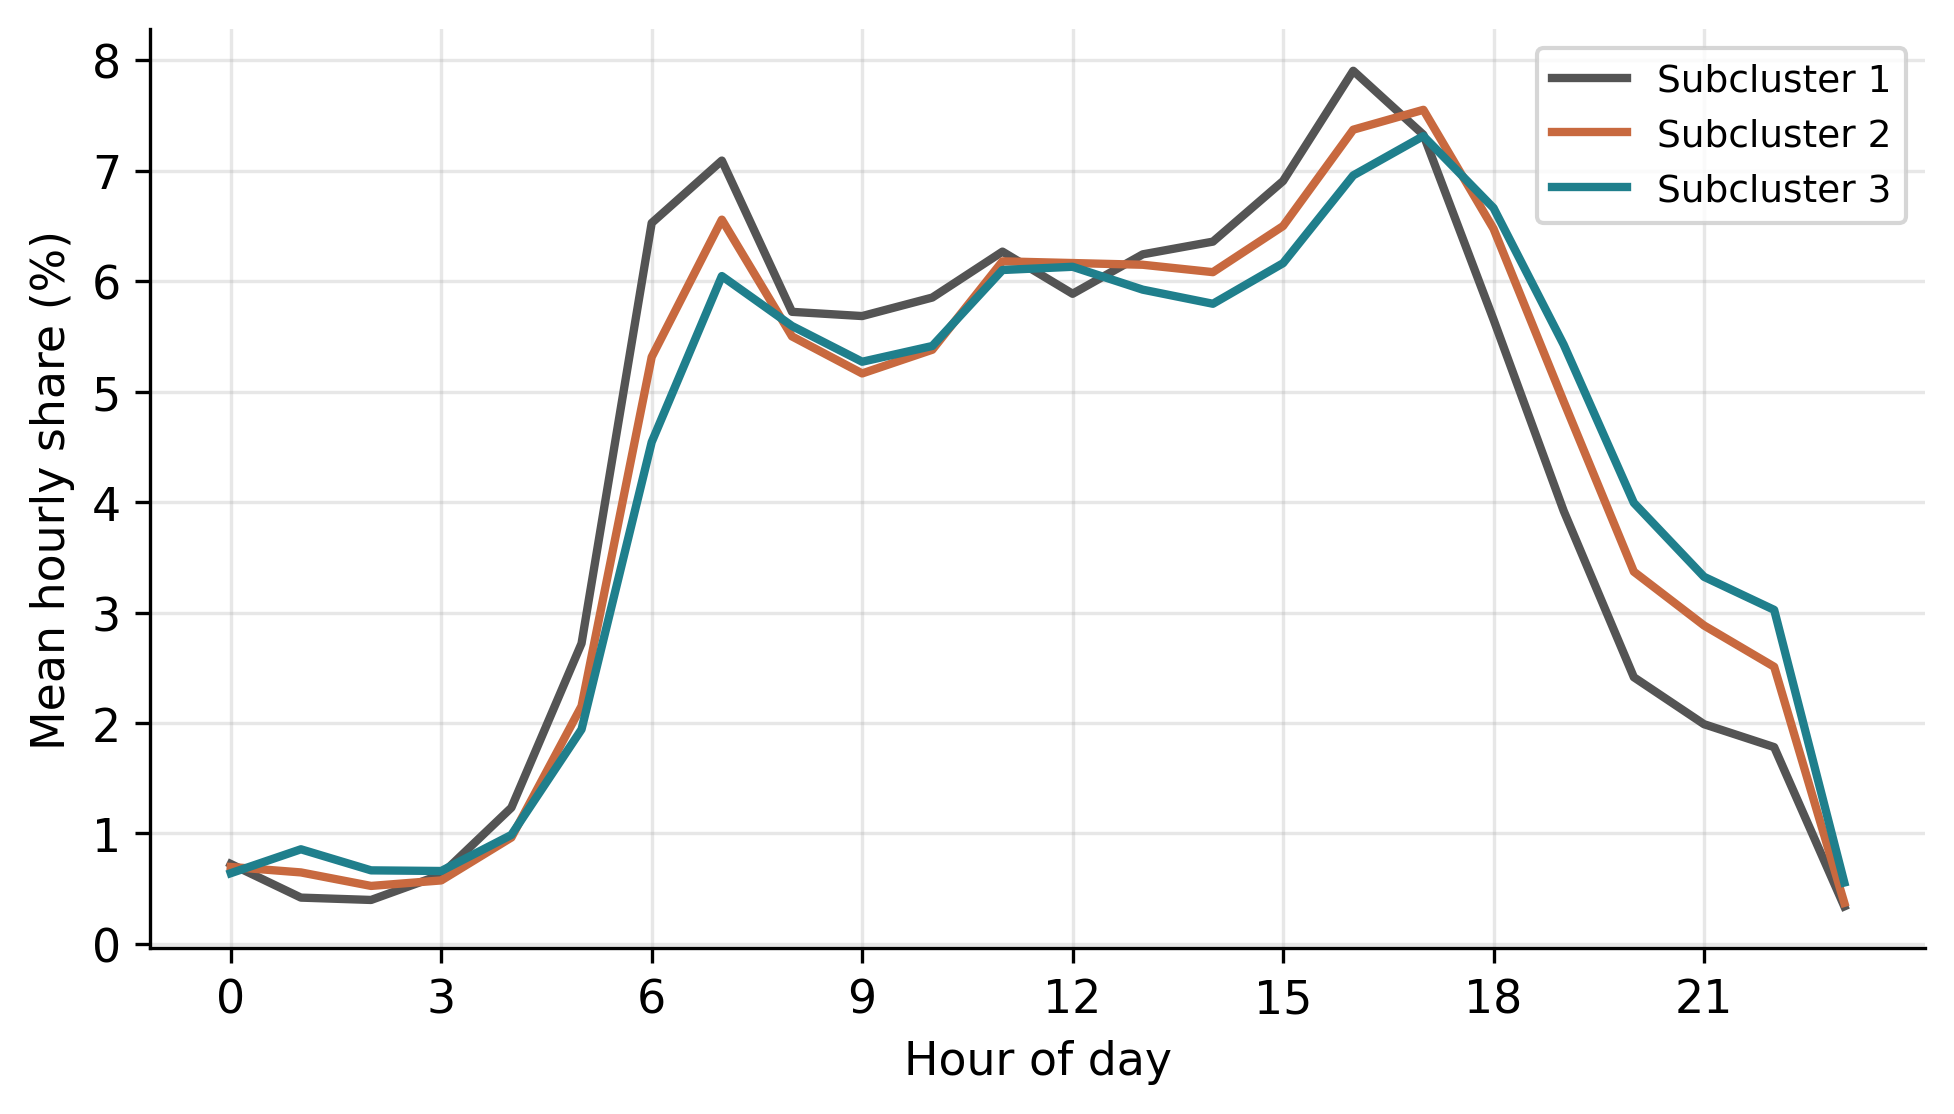
\includegraphics[width=0.7\textwidth]{S_subcluster_profiles.png}
  \caption{Mean normalized simulated profile of the three subclusters of Fig.~8 of the main text (51, 78 and 358 links).}
  \label{fig:subcluster_profiles}
\end{figure}

The selection of the example links in Table~\ref{tab:representatives} follows three rules. The three roads belong to different subclusters. Polyline 104671 is fixed because its position near Forlimpopoli gives it a direct interpretation. In the other two subclusters, among the links with at least 300 simulated vehicles per day and 50 Viasat probes in the week (all 487 candidates), we take the pair with the lowest total MAE whose pairwise distances, including the distance to 104671, are at least 40~km. The two selected links are thus among the best of the candidate set, as the last column of Table~\ref{tab:representatives} shows; the full distribution is in Table~1 and Fig.~10 of the main text.

\begin{table}[htbp]
\centering
\caption{Candidate-filtering logic for the representative validation links.}
\label{tab:representative-candidate-filter}
\begin{tabular}{@{}lrl@{}}
\toprule
Selection stage & Links & Purpose \\
\midrule
Common simulated--Viasat links in 2020 & 930 & Initial matched comparison set. \\
Usable hourly profiles & 848 & Non-zero simulated and GPS totals. \\
Upper $k$-means class of $\log_{10}\eta_i$ & 487 & Candidates for subclustering, $\eta_i\ge0.40\%$. \\
Displayed representative links & 3 & One illustrative link per temporal subcluster. \\
\bottomrule
\end{tabular}
\end{table}

\begin{table}[htbp]
\centering
\caption{Representative polylines of Fig.~9 in the main text. The last column is the percentage of the 848 usable 2020 links with a lower MAE. Minimum pairwise separation: 45.0~km.}
\label{tab:representatives}
\begin{tabular}{@{}rrrrr@{}}
\toprule
Subcluster & Polyline & MAE [pp] & $\varepsilon$ [\%] & Links with lower MAE [\%] \\
\midrule
1 & 104671 & 1.22 & 29 & 40 \\
2 & 134419 & 0.81 & 19 & 5 \\
3 & 64544 & 0.72 & 17 & 1 \\
\bottomrule
\end{tabular}
\end{table}


\section{Aggregate Road-safety Context}
\label{sec:aggregate-safety}

\begin{figure}[htbp]
  \centering
  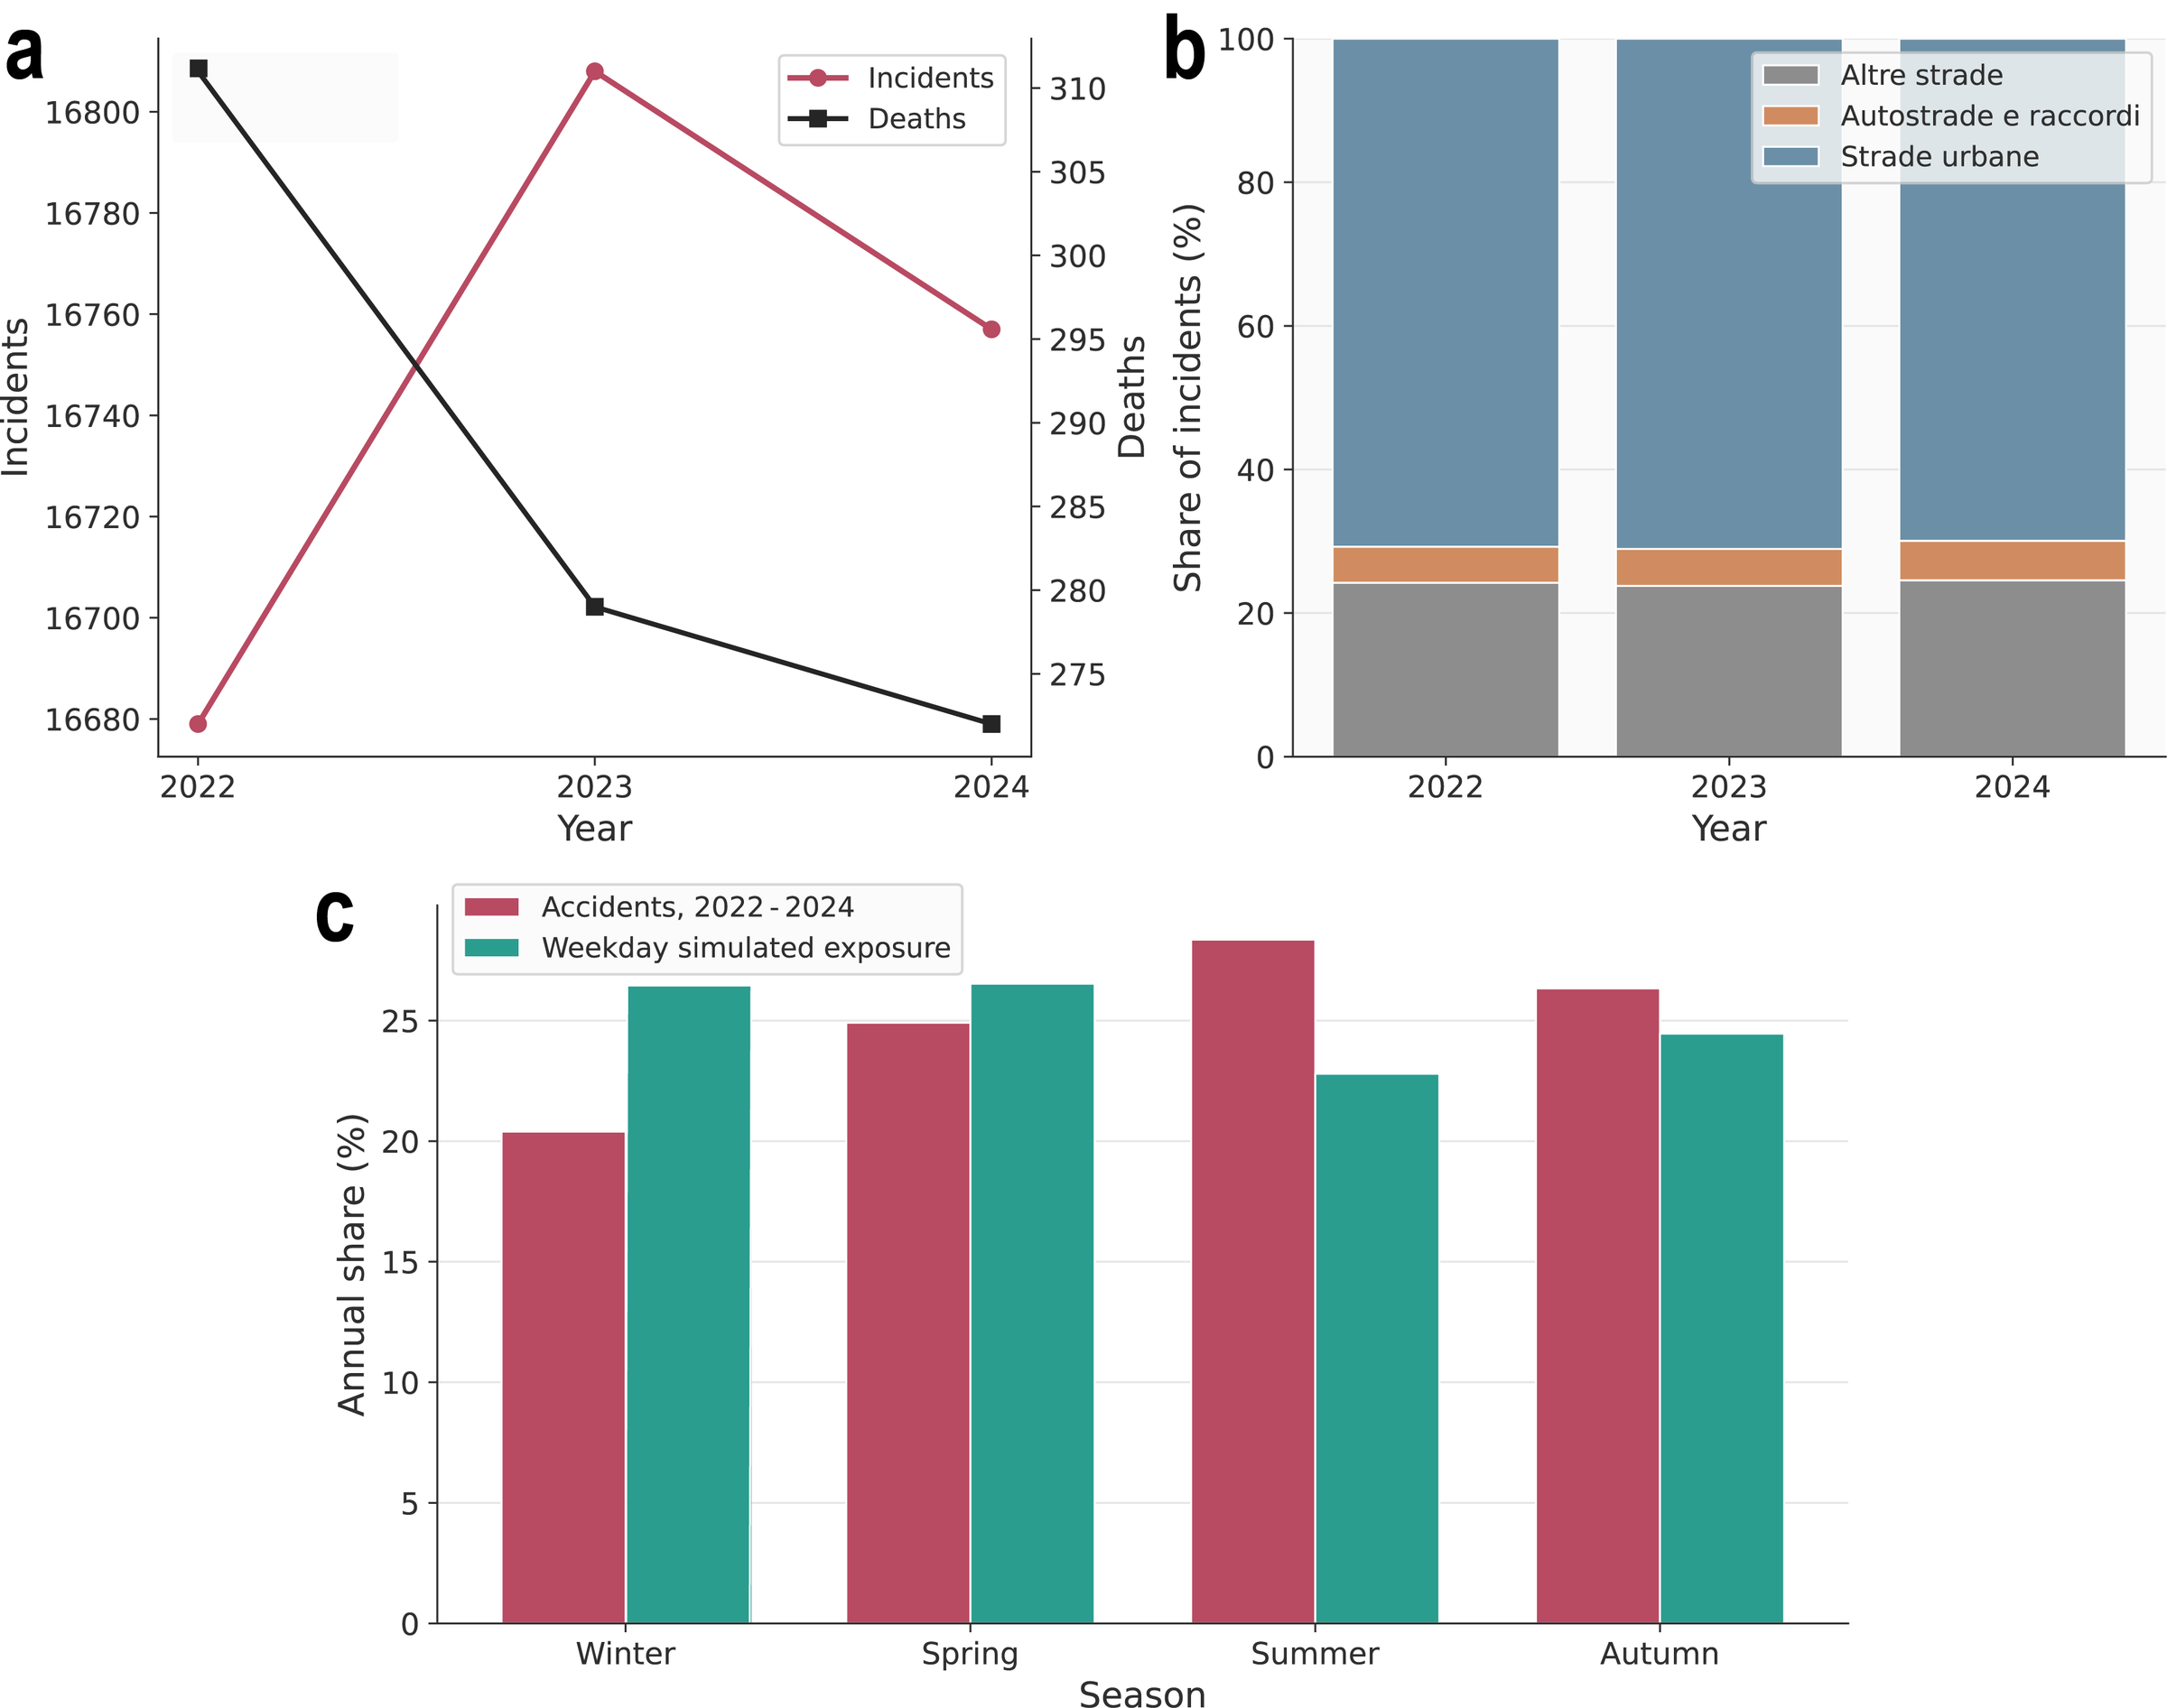
\includegraphics[width=\textwidth]{figsupp.png}
  \caption{Supplementary overview of the accident data used for the
  exposure-normalized road-safety screening. The panels summarize aggregate
  accident totals, road-environment composition and seasonal shares. These
  descriptors are used to contextualize the main-text exposure analysis; they
  are not interpreted as geolocated single-event hotspots.}
  \label{fig:supp_accidents}
\end{figure}

Figure~\ref{fig:supp_accidents} summarizes the aggregate accident context used to interpret the exposure-based safety analyses presented in the main manuscript. The objective of this figure is not to identify geolocated crash hotspots, but to characterize the temporal and infrastructural structure of the regional accident dataset before combining it with reconstructed traffic exposure.

Panel~\textbf{a} reports the total number of recorded accidents and deaths between 2022 and 2024. The total accident count remains relatively stable across years, while fatalities show a moderate decrease over the same period. This indicates that the exposure analysis is performed on a temporally consistent regional dataset without large interannual discontinuities.

Panel~\textbf{b} shows the distribution of accidents across road environments. Urban roads account for the majority of events in all years, whereas highways and ramps contribute only a small fraction of the total recorded accidents. This imbalance is important when interpreting exposure-normalized hazard indicators because high-flow extra-urban corridors may carry substantial traffic volumes while still representing a limited share of total accidents.

Panel~\textbf{c} compares the seasonal accident distribution with the reconstructed simulated exposure field. The observed accident share increases during summer and autumn, while the simulated weekday exposure is more concentrated in winter and spring. This mismatch suggests that accident occurrence cannot be explained solely by reconstructed traffic intensity and may also depend on seasonal behavioural, touristic or environmental factors.

The aggregate descriptors shown in Fig.~\ref{fig:supp_accidents} therefore provide the statistical context for the hazard-weighted exposure analyses discussed in the main text and motivate the use of exposure-normalized indicators rather than raw accident counts alone.



\section{Webserver Architecture}
\label{sec:webserver}

The project also implements the reconstruction as an operational web system. The webserver does not change the modelling equations; it wraps the same configuration generator, simulator and data-assimilation procedure into a service that users can launch from a browser. This distinction matters: the webserver is not an additional calibration method, but an operational layer that makes the validated workflow repeatable for users who need maps, tables and downloadable outputs rather than command-line execution.

\begin{table}[htbp]
\centering
\caption{Logical components of the webserver.}
\label{tab:web-components}
\begin{tabularx}{\linewidth}{@{}lX@{}}
\toprule
Component & Function \\
\midrule
Django graphical interface & Authenticated browser interface. It allows a
user to submit a simulation interval, inspect submitted runs, download
results and open interactive maps. \\
FastAPI simulation service & Programmatic backend that receives simulation
requests, generates a run configuration, launches the simulator in a
separate process and exposes status/results endpoints. \\
Configuration generator & Converts requested dates, coil availability and OD
activity into the simulation input used by the backend. \\
Simulation worker & Runs \modelname{} from the generated configuration and
writes status updates while the model advances. \\
Data-assimilation module & Applies the coil-driven data-assimilation step before results
are returned to the user. A special mode returns provincial min--max
intervals for institutional users. \\
Interactive map layer & Renders cartography and simulated fluxes by colouring
road polylines by quantile or by selected result values. \\
MTS monitoring views & Display coil time series, station maps, rankings,
clusters and local anomaly diagnostics. \\
Scheduled data updater & Downloads and converts the public MTS traffic
records into the standardized coil tables consumed by the simulator. \\
Reverse proxy and containers & Provide a deployable service layout with
separate GUI, simulation API, scheduler and web proxy containers. \\
\bottomrule
\end{tabularx}
\end{table}

The separation between interface, simulation service and worker process keeps long simulations from blocking the browser. The graphical interface stores metadata and displays results; the backend validates requests and coordinates simulation and data assimilation; the worker performs the computationally expensive network loading. The scheduled updater is included because the counter layer is not static: new MTS observations must be converted into the standardized format before they can be used for monitoring or data assimilation.

\begin{table}[htbp]
\centering
\caption{End-user workflow implemented by the dashboard.}
\label{tab:web-workflow}
\begin{tabularx}{\linewidth}{@{}rlX@{}}
\toprule
Step & Action & Result \\
\midrule
1 & Choose interval & The browser submits start time, stop time and output
sampling resolution. \\
2 & Create simulation & The backend validates the request, generates a unique
run identifier and builds the configuration. \\
3 & Run asynchronously & The simulation starts in a separate process while
the interface polls progress. \\
4 & Assimilate results & After completion, the backend applies the default
coil-based data-assimilation step or an institutional min--max adjustment. \\
5 & Persist metadata & The interface stores run identifier, user, status,
runtime, completion and result location in the application database. \\
6 & Visualize and export & Users can inspect time profiles, view flux maps
and download data-assimilated link-flow tables. \\
\bottomrule
\end{tabularx}
\end{table}

The workflow in Table~\ref{tab:web-workflow} mirrors the scientific pipeline of the main manuscript. User input defines the temporal window, the backend generates a model configuration, the simulator produces raw flows, the data-assimilation step applies coil information, and the final link-flow table is stored for visualization and export. The asynchronous status query is practical rather than methodological: a regional simulation can take longer than a normal HTTP request, so the interface polls progress instead of waiting for a blocking response.

\begin{table}[htbp]
\centering
\caption{Conceptual API exposed by the simulation backend.}
\label{tab:web-api}
\begin{tabularx}{\linewidth}{@{}lX@{}}
\toprule
Operation & Meaning \\
\midrule
Welcome/status handshake & Returns service availability and version. \\
Simulation submission & Accepts a time interval and creates a simulation
task. \\
Road-graph export & Returns the road graph geometry used by the interface. \\
Progress query & Reports whether a submitted run is running, complete,
invalid or in error. \\
Result query & When requested after completion, applies data assimilation and
returns the reconstructed link-flow table as JSON or CSV. \\
\bottomrule
\end{tabularx}
\end{table}

The conceptual API in Table~\ref{tab:web-api} exposes only operations needed by the workflow. The road-graph export allows the browser to draw the same network used by the simulator. The result query applies data assimilation at delivery time so the downloaded table and visualized map correspond to the data-assimilated reconstruction, not merely to the raw simulation.

\section{Reproducibility Notes}
\label{sec:reproducibility}

The tables above were derived from stored analysis outputs and source-code inspection. No new simulation run is required to reproduce the reported counts, validation summaries or dashboard architecture. The operational dashboard uses the same simulation and data-assimilation logic described in Sections~\ref{sec:model-details} and \ref{sec:post-correction}; it is therefore an interface to the reconstruction workflow rather than a separate model. Values such as the 10 s integration step, hourly output, five-link data-assimilation depth and 40 km separation threshold should therefore be interpreted in context. The first two define the numerical and observational time scales, the data-assimilation depth controls the spatial locality of sensor information, and the last one is a transparent criterion for choosing readable paper examples rather than hidden calibration parameters.

\end{document}
